\documentclass[10pt,border=2pt]{standalone}
\usepackage{mathptmx}
\usepackage{tikz}
\usetikzlibrary{positioning,arrows.meta,calc}
\usepackage{pgfplots}
\pgfplotsset{compat=1.18}
\usepgfplotslibrary{groupplots}
\setlength{\columnwidth}{88.57mm}
\begin{document}
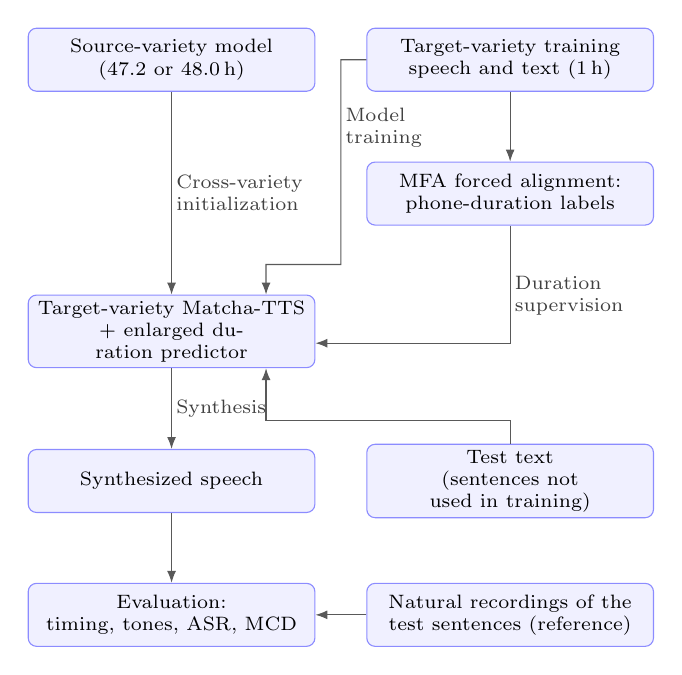
\begin{tikzpicture}[
  font=\scriptsize,
  box/.style={draw=blue!45, rounded corners=3pt, align=center, minimum height=8mm, text width=35mm, inner sep=2pt, fill=blue!6},
  lab/.style={font=\scriptsize, text=black!75, align=left, inner sep=1.5pt},
  arr/.style={-{Latex[length=1.5mm]}, gray!70!black}]
\node[box] (src)   at (0, 0) {Source-variety model\\(47.2 or 48.0\,h)};
\node[box] (train) at (4.3, 0) {Target-variety training\\speech and text (1\,h)};
\node[box] (mfa)   at (4.3, -1.7) {MFA forced alignment:\\phone-duration labels};
\node[box] (tts)   at (0, -3.45) {Target-variety Matcha-TTS\\+ enlarged duration predictor};
\node[box] (syn)   at (0, -5.35) {Synthesized speech};
\node[box] (text)  at (4.3, -5.35) {Test text\\(sentences not used in training)};
\node[box] (eval)  at (0, -7.05) {Evaluation:\\timing, tones, ASR, MCD};
\node[box] (nat)   at (4.3, -7.05) {Natural recordings of the\\test sentences (reference)};
\draw[arr] (train) -- (mfa);
\draw[arr] (src) -- node[lab, right]{Cross-variety\\initialization} (tts);
\draw[arr] (train.west) -- (2.15,0) -- node[lab, right, pos=0.33]{Model\\training} (2.15,-2.6) -- (1.2,-2.6) -- ([xshift=12mm]tts.north);
\draw[arr] (mfa.south) |- node[lab, right, pos=0.3]{Duration\\supervision} ([yshift=-1.5mm]tts.east);
\draw[arr] (tts) -- node[lab, right]{Synthesis} (syn);
\draw[arr] (text.north) -- ++(0,0.3) -| ([xshift=12mm]tts.south);
\draw[arr] (syn) -- (eval);
\draw[arr] (nat) -- (eval);
\end{tikzpicture}
\end{document}
